{\color{blue}
\section{Framework Resources Quantification Model}\label{model}

In this section, we introduce \textit{Framework Resources Quantification} (FRQ) model to describe the performance of DAG frameworks.
The FRQ model quantifies computing and I/O resources and visualizes them in the time dimension. According to the FRQ model, we can calculate the execution time required by the application under any circumstances, including different DAG frameworks, hardware environments, and so on. Therefore the FRQ model is able to help us analyze the resources scheduling of DAG framework and evaluate their performance. We will first introduce the FRQ model in Subsection \ref{model_overview}. In the following Subsection \ref{model_analysis}, we will use the FRQ model to describe three different computation jobs and analyze their performance. In the last Subsection \ref{model_verification}, we will use the actual experimental results to verify the FRQ model.

\subsection{The FRQ Model}\label{model_overview}
The current distributed computing frameworks mostly use DAGs to describe computation logic. 
A shuffle phase is required between each adjacent DAG computation phases. To better analyze the relationship between the computation phase and the shuffle phase, we propose the FRQ model. After quantifying computing and I/O resources, the FRQ model can describe different resource scheduling strategies. For convenience, we introduce the FRQ model by taking a simple MapReduce job as an example in this section.

Figure \ref{fig:model_basic} shows how the FRQ model describes a MapReduce task. The FRQ model has five input parameters:
\begin{itemize}
	\item Input Data Size \((D)\): The data size of the computation phase.
	\item Data Conversion Rate \((R)\): The conversion rate of the input data to the shuffle data during a computation phase. This rate depends on the algorithm used in the computation phase.
    \item Computation Round Number \((N)\): The number of rounds needed to complete the computation phase. These rounds depend on the current computation resources and the configuration of the framework. Take Hadoop MapReduce as an example. Suppose we have a cluster with 50 CPUs and enough memory, the map phase consists of 200 map tasks, and each map requires 1 CPU. Then we need 4 rounds of computation to complete the map phase.
    \item Computation Speed \((V_{i})\): 
    The computation speed for each computation phase. This speed depends on the algorithm used in the computation phase.
    \item Shuffle Speed \((V_{Shuffle})\): 
    Transmission speed in the shuffle phase. This speed depends on network and storage device bandwidth.
\end{itemize}

\begin{figure*}
    \centering
	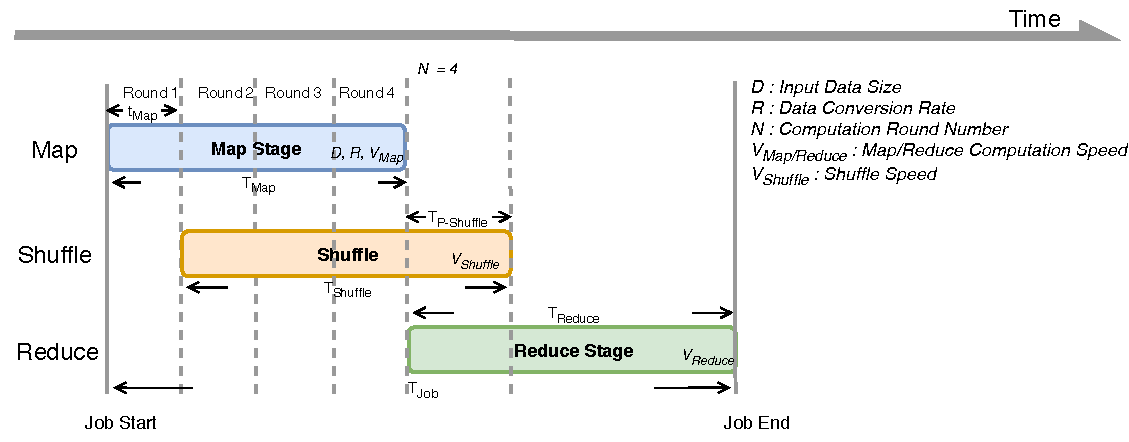
\includegraphics[width=0.85\textwidth]{fig/model_basic}
	\caption{\color{blue}Framework Resources Quantification (FRQ) Model with Full Parallel MapReduce}
    \label{fig:model_basic}
    \vspace{-1em}
\end{figure*}
The FRQ model calculates the execution time of each phase of the job with these five parameters. As shown in Figure \ref{fig:model_basic}, the total execution time of a job is the sum of the map phase time and reduce phase time:
\begin{equation}
\label{equation_Tjob}
\begin{aligned}
    T_{Job} &= T_{Map} + T_{Reduce}
\end{aligned}
\end{equation}

Map phase time depends on input data size and map computation speed:
\begin{equation}
\label{equation_Tmap}
\begin{aligned}
    T_{Map} &= {{\frac{D}{V_{Map}}}}
\end{aligned}
\end{equation}

The reduce phase time formula is as follows:
\begin{equation}
\label{equation_Treduce}
\begin{aligned}
    T_{Reduce} &= \frac{D \times R}{V_{Reduce}} + K \times T_{P\_Shuffle}
\end{aligned}
\end{equation}

\(\frac{D \times R}{V_{Reduce}}\) represents the ideal computation time of a reduce phase, and (\(K \times T_{P\_Shuffle}\)) represents the computing overhead.
We use \(T_{P\_Shuffle}\) to represent the overlap time between shuffle phase and reduce phase. \(T_{Shuffle}\) represents the total time of the shuffle phase. 
The relationship between \(T_{P\_Shuffle}\) and \(T_{Shuffle}\) is determined by the resources scheduling strategy of DAG frameworks. This relationship will be shown in the following Subsection \ref{model_analysis}.  
\(K\) is an empirical value. 
Because the computation of the reduce phase relies on the data transfer results of the shuffle phase, a portion of the computation in the reduce phase needs to wait for the transfer results. This waiting causes the overhead. The FRQ model uses K to indicate the extent of the waiting.

The shuffle phase time formula is as follows:
\begin{equation}
\label{equation_Tshuffle}
\begin{aligned}
    T_{Shuffle} &= {{\frac{D}{V_{Shuffle}}}}
\end{aligned}
\end{equation}

According to Equation \ref{equation_Tjob}\&\ref{equation_Treduce}, we can optimize the job completion time by reducing \(T_{P\_Shuffle}\). Improving I/O speed is an effective way to reduce shuffle time. Another optimization method is to use the idle I/O resources in the map phase for pre-fetching (see Figure \ref{fig:model_basic}). Both of the above methods can effectively reduce \(T_{P\_Shuffle}\). 
By using the FRQ model to describe a MapReduce job, the users can analyze the resource scheduling strategy of the computation framework.

\subsection{Model Analysis}\label{model_analysis}

\begin{figure*}
	\centering
	\begin{subfigure}{0.47\linewidth}
		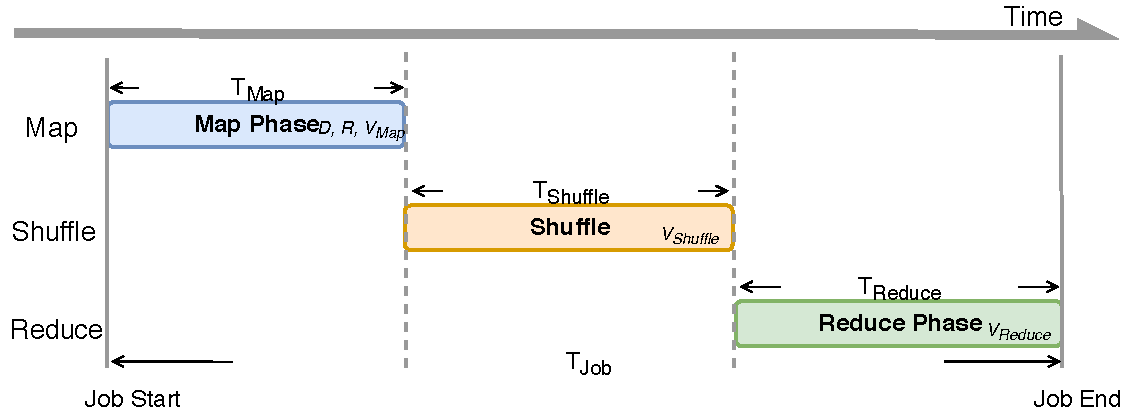
\includegraphics[width=\linewidth]{fig/model_original}
		\caption{\color{blue}Full Serial MapReduce}
		\label{fig:model_original}
	\end{subfigure}
	\begin{subfigure}{0.47\linewidth}
		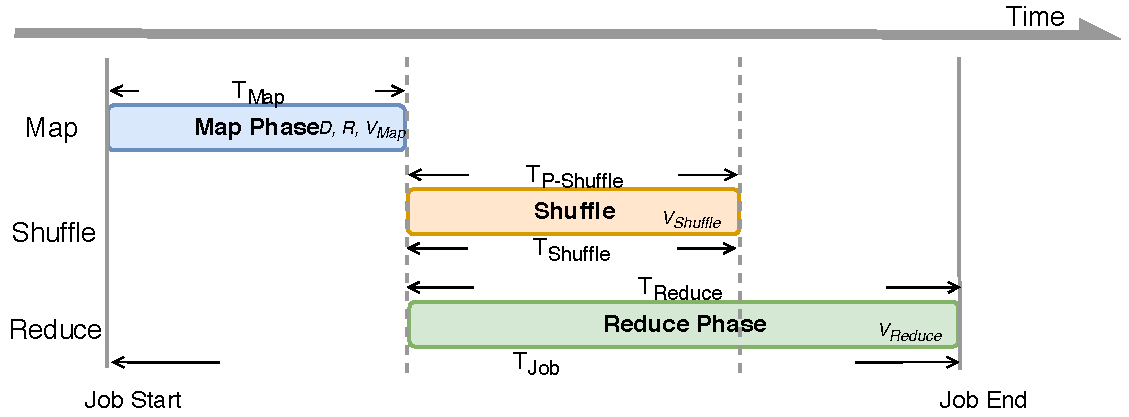
\includegraphics[width=\linewidth]{fig/model_hadoop}
		\caption{\color{blue}Half Parallel MapReduce}
		\label{fig:model_hadoop}
	\end{subfigure}
	\caption{\color{blue}Framework Resources Quantification (FRQ) Model with Different Scheduling Strategies}
	\label{fig:model_strategies}
\end{figure*}

The FRQ model can describe a variety of resource scheduling strategies. First, we analyze a simple scheduling strategy which used by Apache Spark by default. 
As shown in Figure \ref{fig:model_original}, the FRQ model describes a MapReduce job that is entirely serially executed. The overlap time between the shuffle phase and the reduce phase is \(0\), in which case \(T_{P\_Shuffle}\) is \(0\). Therefore, the overhead of the reduce phase is 0. The total execution time of a job is also different from the above:
\begin{equation}
\label{equation_Tjob2}
\begin{aligned}
    T_{Job} &= T_{Map} + T_{Shuffle} + T_{Reduce}
\end{aligned}
\end{equation}

Due to serialization, the I/O resource is idle during the reduce phase and map phase. This scheduling strategy is simple and has much room for optimization.

Figure \ref{fig:model_hadoop} shows a more efficient scheduling strategy which is used by Hadoop MapReduce. In this scheduling strategy, shuffle phase and reduce phase start at the same time. In this case, \(T_{P\_Shuffle}\) is equal to \(T_{Shuffle}\). Due to the increase in \(T_{P\_Shuffle}\), the time of reduce phase increases (according to Equation \ref{equation_Treduce}). Because the shuffle phase and the computation phase are executed in parallel, the total execution time of a job is the sum of \(T_{Map}\) and \(T_{Reduce}\) (see Equation \ref{equation_Tjob}). The execution time of the shuffle phase is hidden in the reduce phase. 
However, we also found that the I/O resource in the map phase is still idle. This scheduling strategy can still be optimized.

\begin{figure*}
	\centering
	\begin{subfigure}{0.47\linewidth}
		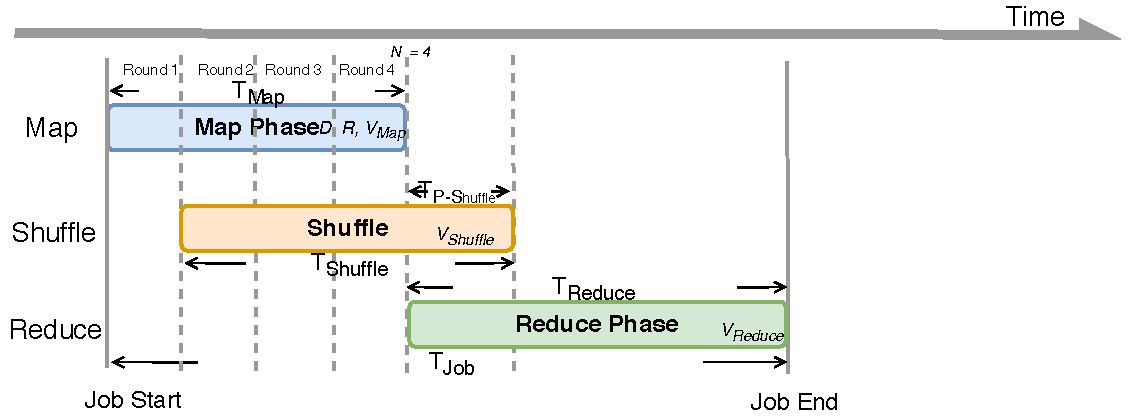
\includegraphics[width=\linewidth]{fig/model_scache1}
		\caption{\color{blue}If \(V_{Map} \times R \ge V_{Shuffle}\)}
		\label{fig:model_scache1}
	\end{subfigure}
	\begin{subfigure}{0.47\linewidth}
		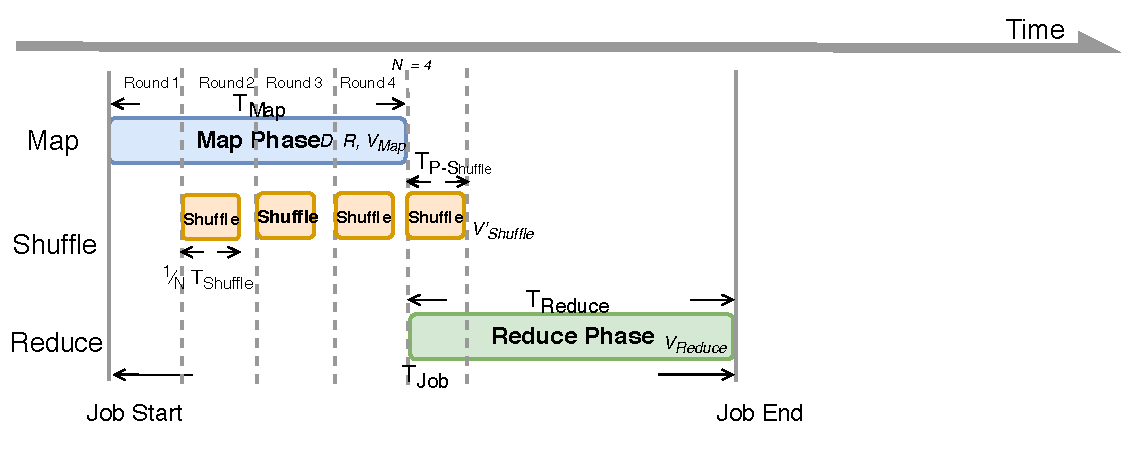
\includegraphics[width=\linewidth]{fig/model_scache2}
		\caption{\color{blue}If \(V_{Map} \times R < V_{Shuffle}\)}
		\label{fig:model_scache2}
	\end{subfigure}
	\caption{\color{blue}Framework Resources Quantification (FRQ) Model with Full Parallel MapReduce in Different Environments}
	\label{fig:model_scache}
\end{figure*}

Hadoop MapReduce overlaps shuffle phase with reduce phase and utilizes idle resources. We intuitively think that we can also overlap shuffle phase one and map phases. We implemented this idea with SCache.
Figure \ref{fig:model_scache} shows the scheduling strategy for Hadoop MapReduce with SCache (Suppose N is 4). SCache starts pre-fetching and pre-scheduling in the map phase. This scheduling strategy can make better use of resources and avoid the I/O resource being idle in the map phase. According to the design of SCache pre-fetching, we found that using the FRQ model to describe the scheduling strategy of SCache needs to distinguish two situations:

\begin{enumerate}
    \item 
    \(V_{Map} \times R \ge V_{Shuffle}\) (Figure \ref{fig:model_scache1}): 
	The meaning of the inequality is that the speed of generating shuffle data (\(V_{Map} \times R\)) is greater than or equal to the shuffle speed (\(V_{Shuffle}\)). 
	In this situation, the shuffle phase is uninterrupted. The I/O resource will be fully utilized during the whole shuffle phase. As a result, the formula of \(T_{PShuffle}\) is as followed:
	\begin{equation}
		\label{equation_Tpshuffle1}
		\begin{aligned}
			T_{P\_Shuffle} &= T_{Shuffle} - \frac{(N - 1)\times T_{Map}}{N}
		\end{aligned}
	\end{equation}
	
    \item \(V_{Map} \times R < V_{Shuffle}\) (Figure \ref{fig:model_scache2}): 
	When the shuffle speed (\(V_{Shuffle}\)) is faster, SCache needs to wait for shuffle data to be generated. As Figure \ref{fig:model_scache2} shown, the shuffle phase will be interrupted in each round. In this case, the formula of \(T_{PShuffle}\) is as followed:
	\begin{equation}
		\label{equation_Tpshuffle2}
		\begin{aligned}
			T_{P\_Shuffle} &= T_{Shuffle} \times \frac{1}{N}
		\end{aligned}
	\end{equation}
\end{enumerate}

Compared to the original Hadoop MapReduce resource scheduling strategy, Hadoop MapReduce with SCache shortens \(T_{P\_Shuffle}\) and thus shortens \(T_{Reduce}\). This is how pre-fetching optimizes the total execution time of a job.

% \begin{table}[!t]
\begin{table*}
\centering
\scalebox{0.91}{
	\begin{tabular}{|c||c|c|c|c|c|c|c||c|c|c|c|c|c|c|}
	\hline
	&
	\(D\) &	
	\(R\) &	
	\(N\) &	
	\(V_{Map}\) &	
	\(V_{Reduce}\) &	
	\(V_{Shuffle}\) &	
	\(K\) &	
	\(T_{Map}\) &	
	\(T_{Shuffle}\) &	
	\(T_{P\_Shuffle}\) &
	\(T_{Reduce}\) & 
	\(T_{Job}\) & 
	\(Exp T_{Job}\) &
	\(Error\)\\

	\hline
	& 16	& 1	& 2 &	0.65 &	1 &	0.47 &	0.5 &	24.62 &		34.04	 &	21.73 &	26.87 &	51.48	& 55  &		6.39\% \\
	SCache
	& 32	& 1	& 4 &	0.65 &	1 &	0.47 &	0.5 &	49.23 &		68.09	 &	31.16 &	47.58 &	96.81	& 104 & 	6.91\% \\
	& 48	& 1	& 6 &	0.65 &	1 &	0.47 &	0.5 &	73.85 &		102.13 &	40.59 &	68.29 &	142.14	& 151 & 	5.87\% \\
	& 64	& 1	& 8 &	0.65 &	1 &	0.47 &	0.5 &	98.46 &		136.17 &	50.02 &	89.01 &	187.47	& 193 & 	2.87\% \\
	\hline
	& 16	& 1 & 2 &	0.65 &	1 &	0.47 &	0.6 &	24.62 &		34.04	&	34.04	&	36.43	&	61.04	&	73	&	16.38\%	\\
	Legacy
	& 32	& 1 & 4 &	0.65 &	1 &	0.47 &	0.6 &	49.23 &		68.09	&	68.09	&	72.85	&	122.08	&	135	&	9.57\%	\\
	& 48	& 1 & 6 &	0.65 &	1 &	0.47 &	0.6 &	73.85 &		102.13	&	102.13	&	109.28	&	183.12	&	188	&	2.59\%	\\
	& 64	& 1 & 8 &	0.65 &	1 &	0.47 &	0.6 &	98.46 &		136.17	&	136.17	&	145.70	&	244.16	&	249	&	1.94\%	\\
	\hline
	\end{tabular}
}
\(D\): GB, \(V_{i}\): GB/s, \(T_{i}\): s
\caption{\color{blue}Hadoop MapReduce on 4 nodes cluster in the FRQ model}
\label{table1}
\end{table*}
% \subsection{Performance Analysis}\label{model_performance_analysis}

% \begin{table*}[!t]
\begin{table*}
\centering
\scalebox{0.9}{
	\begin{tabular}{|c||c|c|c|c|c|c|c||c|c|c|c|c|c|c|}
	\hline
	&
	\(D\) &	
	\(R\) &	
	\(N\) &	
	\(V_{Map}\) &	
	\(V_{Reduce}\) &	
	\(V_{Shuffle}\) &	
	\(K\) &	
	\(T_{Map}\) &	
	\(T_{Shuffle}\) &	
	\(T_{P\_Shuffle}\) &
	\(T_{Reduce}\) & 
	\(T_{Job}\) & 
	\(Exp T_{Job}\) &
	\(Error\)\\

	\hline
	& 128	& 1 & 5 &	1.15 &	1.46	&	1.4 &	0.5 &	111.30 &	91.43	&	18.29	&	96.81	&	208.12	&	232	&	10.29\%	\\
	SCache
	& 256	& 1 & 5 &	1.15 &	1.46	&	1.4 &	0.5 &	222.61 &	182.86	&	36.57	&	193.63	&	416.24	&	432	&	3.65\%	\\
	& 384	& 1 & 5 &	1.15 &	1.46	&	1.4 &	0.5 &	333.91 &	274.29	&	54.86	&	290.44	&	624.36	&	685 &	8.85\%	\\
	% & 512	& 1 & 5 &	1.15 &	1.46	&	1.4 &	0.5 &	445.22 &	365.71	&	91.43	&			&	841.62	&	1135 &	25.85\%	\\
	\hline
	& 128	& 1 & 5 &	1.15 &	1.46	&	1.4 &	0.6 &	111.30 &	91.43	&	91.43	&	142.53	&	253.83	&	266 &	4.57\%	\\
	Legacy
	& 256	& 1 & 5 &	1.15 &	1.46	&	1.4 &	0.6 &	222.61 &	182.86	&	182.86	&	285.06	&	507.67	&	524 &	3.12\%	\\
	& 384	& 1 & 5 &	1.15 &	1.46	&	1.4 &	0.6 &	333.91 &	274.29	&	274.29	&	427.59	&	761.50	&	776 &	1.87\%	\\
	% & 512	& 1 & 5 &	1.15 &	1.46	&	1.4 &	0.6 &	445.22 &	365.71	&	365.71	&	588.40	&	1033.62	&	1312 &	21.22\%	\\

	\hline
	\end{tabular}
}
\(D\): GB, \(V_{i}\): GB/s, \(T_{i}\): s
\caption{\color{blue}Hadoop MapReduce on 50 AWS m4.xlarge nodes cluster in the FRQ model}
\label{table2}
\end{table*}

\subsection{Model Verification}\label{model_verification}
To verify the FRQ model, we run experiments on two environments: (a) 50 Amazon EC2 m4.xlarge nodes cluster as shown in Subsection \ref{stepup}. (b) 4 in-house nodes cluster with 128GB memory and 32 cores per node. To simplify the calculation of the FRQ model, we run the Terasort as an experimental application on a Hadoop MapReduce framework. We deployed Hadoop with SCache and without SCache in both environments.

Table \ref{table1} shows the calculational results of the FRQ model in the in-house environment. The workload is from 16 GB to 64 GB. 
\(D\) and \(N\) are set according to the application parameters. \(R, V_{Map}, V_{Shuffle},\)and \(V_{Reduce}\) are calculated based on experimental results. K is the empirical value, we set \(K\) to 0.5 and 0.6, which reflects that \(T_{P\_Shuffle}\) has less impact on the reduce phase in the case of SCache. 
% The formulas of \(T_{Job}, T_{Map}, T_{Reduce}\) and \(T_{Shuffle}\) are according to Equation \ref{equation_Tjob}, Equation \ref{equation_Tmap}, Equation \ref{equation_Treduce} and Equation \ref{equation_Tshuffle}, respectively. 
In the Hadoop with SCache, Terasort satisfies the situation in Figure \ref{fig:model_scache1} (\(V_{Map} \times R \ge V_{Shuffle}\)). 
% thus the formula of \(T_{P\_Shuffle}\) is Equation \ref{equation_Tpshuffle1}.
In the original Hadoop, since pre-fetching is not used, \(T_{P\_Shuffle}\) is equal to \(T_{Shuffle}\)(see Equation \ref{equation_Tshuffle}). \(ExpT_{Job}\) represents the actual experiment data, we calculate \(Error\) according to \(T_{Job}\) and \(ExpT_{Job}\). 
% The formula of \(Error\) is:
% \begin{equation}
% 	\label{equation_error}
% 	\begin{aligned}
% 		Error &= \frac{ExpT_{Job} - T_{Job}}{T_{Job}}
% 	\end{aligned}
% \end{equation}

Table \ref{table2} shows the calculational results of the FRQ model in Amazon EC2 environment. \;\(V_{Map}, V_{Shuffle},\) and \(V_{Reduce}\) are modified because of the different hardware devices. We also set K to the same empirical value. The formulas in the table are all the same except \(T_{P\_Shuffle}\). In this environment, Terasort on Hadoop MapReduce satisfies the situation in Figure \ref{fig:model_scache2} (\(V_{Map} \times R < V_{Shuffle}\)), thus the formula of \(T_{P\_Shuffle}\) is Equation \ref{equation_Tpshuffle2}. 
% In the previous case, \(T_{P\_Shuffle}\) is still equal to \(T_{Shuffle}\).

\begin{figure*}
	\centering
	\begin{subfigure}{.42\linewidth}
		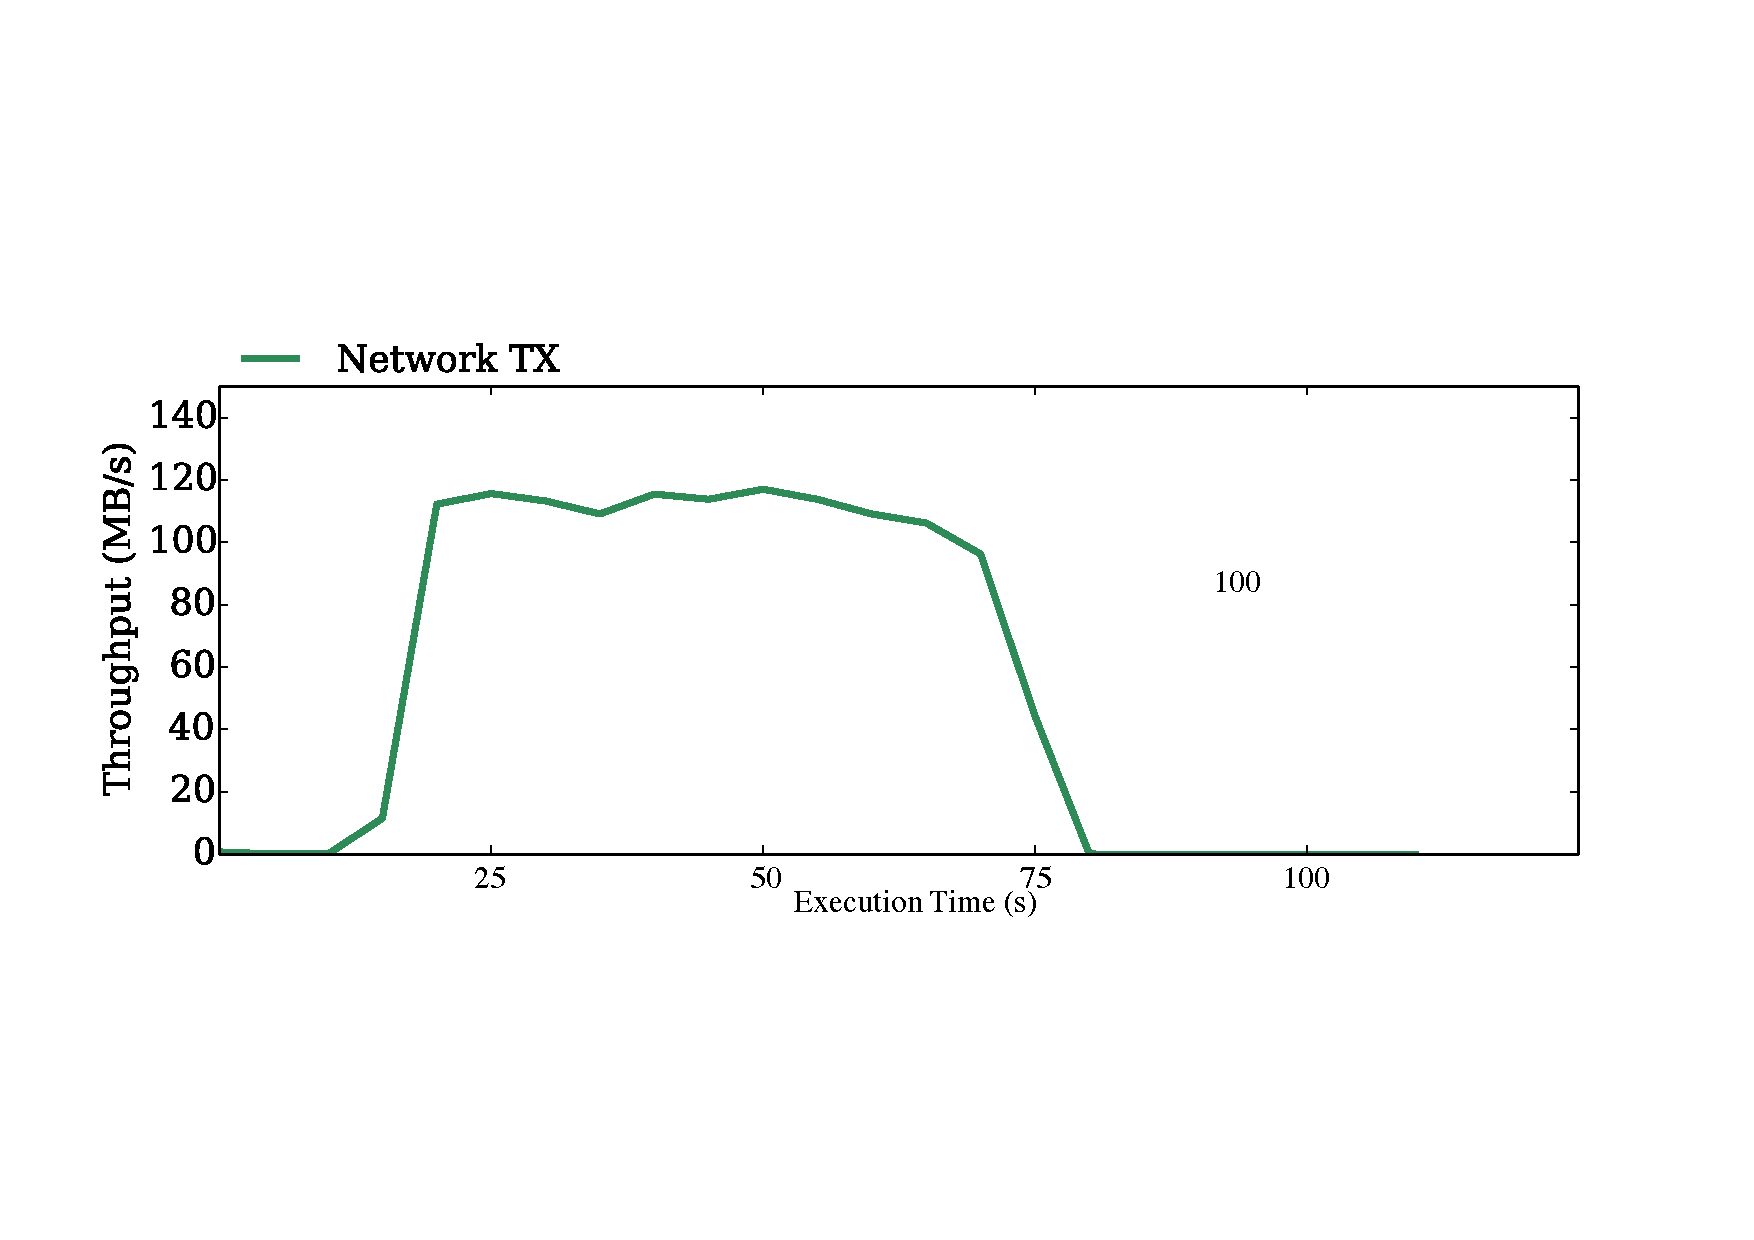
\includegraphics[width=\linewidth]{fig/hadoop_net1}
		\caption{\color{blue}If \(V_{Map} \times R \ge V_{Shuffle}\)}
		\label{fig:hadoop_net1}
	\end{subfigure}
	\begin{subfigure}{.42\linewidth}
		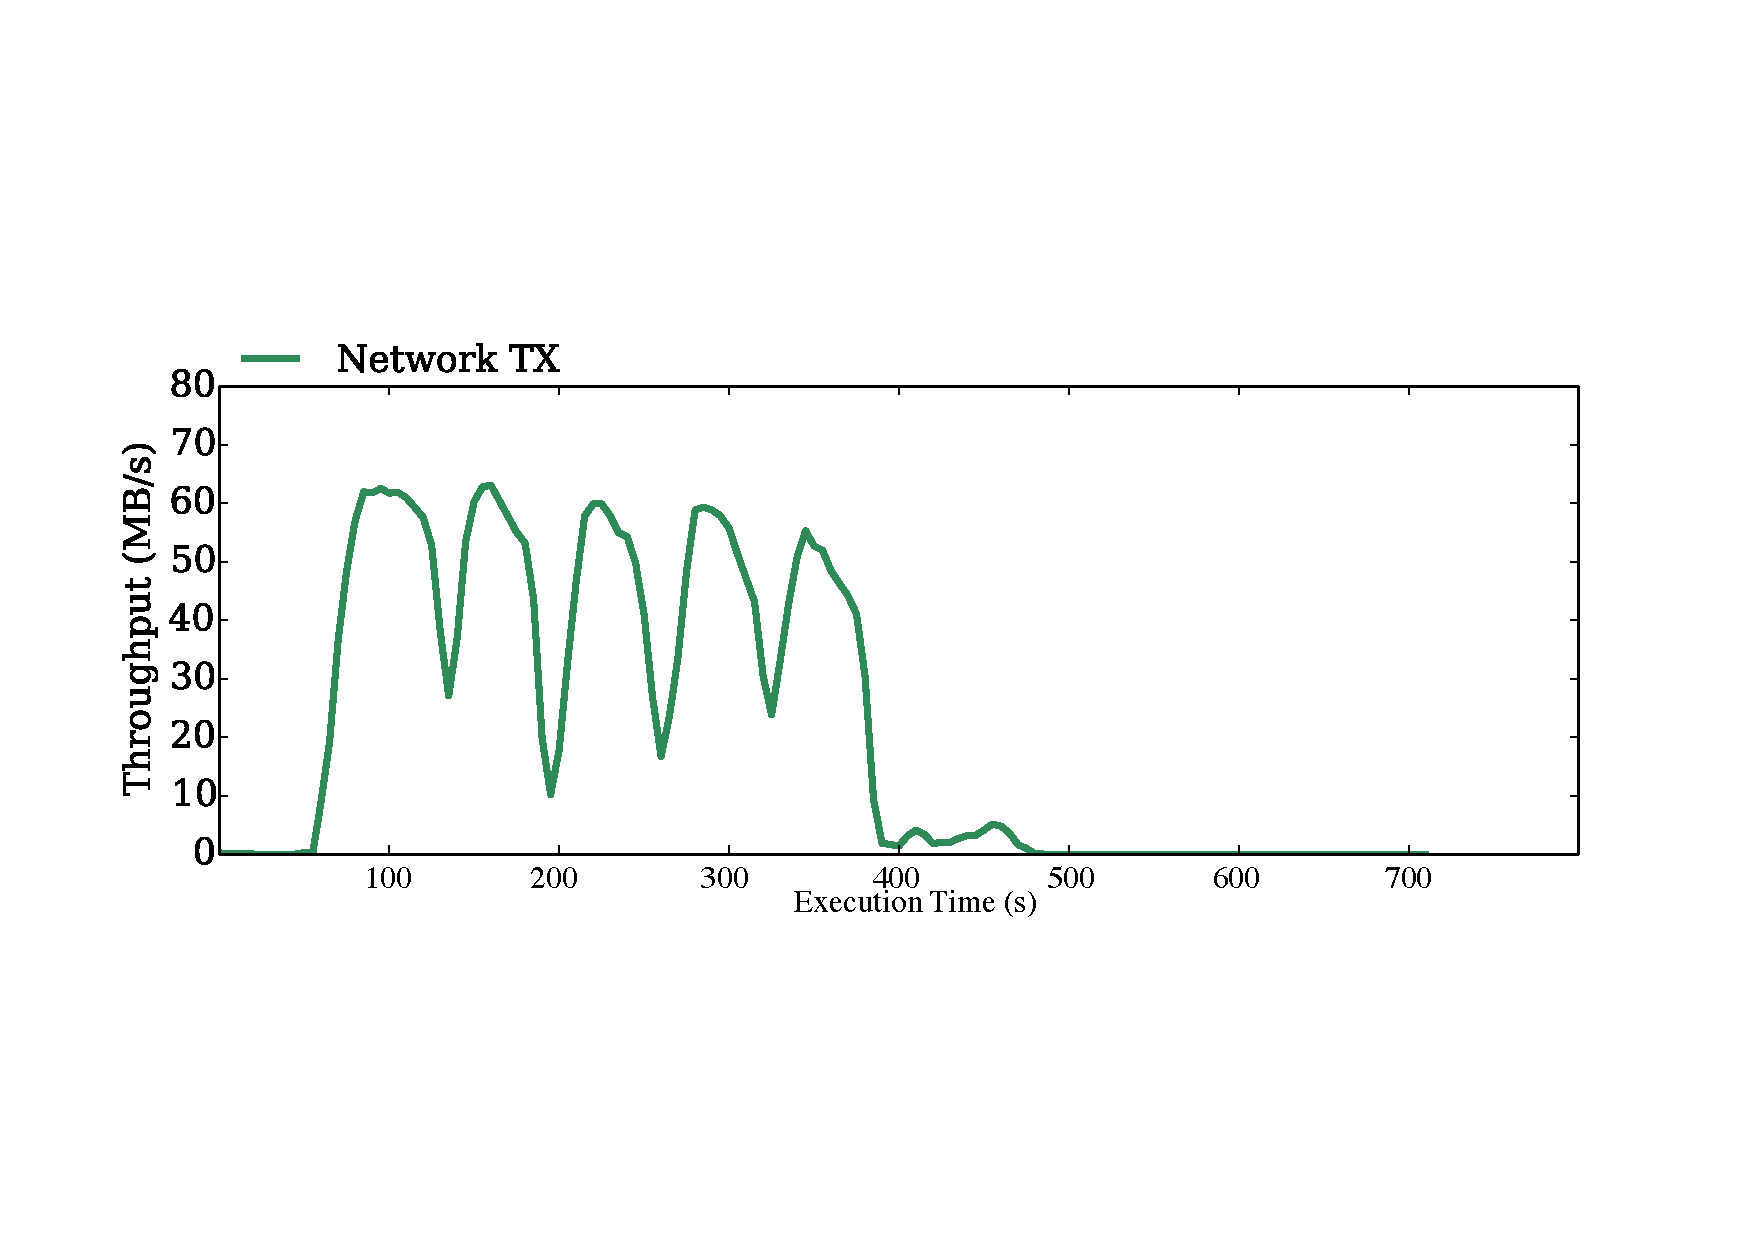
\includegraphics[width=\linewidth]{fig/hadoop_net2}
		\caption{\color{blue}If \(V_{Map} \times R < V_{Shuffle}\)}
		\label{fig:hadoop_net2}
	\end{subfigure}
	\caption{\color{blue}Network utilization on Hadoop MapReduce with SCache}
	\label{fig:hadoop_net}
\end{figure*}

In order to verify the two cases as mentioned above when using SCache, we monitor the network utilization as Figure \ref{fig:hadoop_net}. Figure \ref{fig:hadoop_net1} shows that, in the in-house environment, the network utilization remains high until the shuffle phase is completed. On the other hand, Figure \ref{fig:hadoop_net2} shows that the network utilization has 5 regular peaks in Amazon EC2 environment. 
Both these two situations are consistent with the FRQ model in Figure \ref{fig:model_scache}. 
% Therefore, we believe that the FRQ model is able to accurately describe the performance of a framework with SCache.

Regarding accuracy, the experimental values are all larger than the calculated values. This is because the application has some extra overhead at runtime, such as network warm-up, the overhead of allocating slots, and so on. 
% In the case where the input data is small and the total time is short, the error caused by the overhead is amplified. 
This overhead will be amplified when the input data is small or the total execution time is short. 
Overall, the error between \(T_{Job}\) and \(ExpT_{Job}\) is mainly below 10\%, such errors are acceptable. Therefore, we believe that the FRQ model can accurately describe DAG frameworks.
}